%!TEX root = ../../thesis.tex

\cite{MCnet:general}

Monte Carlo method

\subsection{The anatomy of an event}

\begin{figure}
	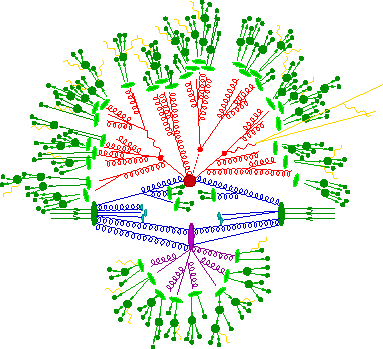
\includegraphics[width=\largefigwidth]{tex/tools/event}
	\caption{Schematic diagram of a simulated \ttH event, showing how factorisation allows 
	the physics at different scales of momentum transfer $Q$ to be treated independently.
	At high-$Q^2$ is the hard scatter (red circle). As the scale evolves down, partons are 
	radiated in the initial state (blue) and final state (red). At low-$Q^2$, incoming 
	partons are confined to the beam protons, while outgoing partons hadronise (light 
	green blobs). The underlying event contains multiple partonic interactions (purple 
	blob) and beam remnants (light blue blobs). Photons (yellow) are also radiated.}
	\label{fig:mcevent}
\end{figure}

\begin{description}
\item[Hard subprocess] \hfill \\
	perturbative QCD, process dependent
\item[\acp{PDF}] \hfill \\
	non-perturbative
\item[\ac{FSR}] \hfill \\
	dumdeedoo
\item[\ac{ISR}] \hfill \\
	dumdeedoo
\item[Hadronisation] \hfill \\
	non-perturbative, cluster and Lund string models
\item[Hadronic decay] \hfill \\
	dumdeedoo
\item[\ac{MPI}] \hfill \\
	process dependent, non-perturbative, various models
\item[\acs{QED} radiation] \hfill \\
	dumdeedoo
\end{description}

\subsection{Summary of event generators}
\begin{description}
\item[Herwig] \hfill \\
	\fherwig or \herwigpp \cpp
\item[Pythia] \hfill \\
	\pythia{6} or \pythia{8}
\item[\sherpa] \hfill \\
	\sherpa
\end{description}

\subsection{ME-PS merging}
\begin{description}
\item[CKKW] \hfill \\
	dumdeedoo
\item[MLM] \hfill \\
	dumdeedoo
\end{description}

\subsection{NLO-PS matching}
\begin{description}
\item[\mcatnlo] \hfill \\
	dumdeedoo
\item[\powheg] \hfill \\
	dumdeedoo
\end{description}

\subsection{Additional considerations}
\begin{description}
\item[Pile-up] \hfill \\
	in-time/out-of-time pile-up
\item[Detector simulation] \hfill \\
	GEANT4
\end{description}